%%%%%%%%%%%%%%%%%%%%%%%%%%%%%%%%%%%%%%%%%%%%%%%%%%%%%%%%%%%%%%%%%%%%%%%%%%%%%%%%%%%%
% Document data
%%%%%%%%%%%%%%%%%%%%%%%%%%%%%%%%%%%%%%%%%%%%%%%%%%%%%%%%%%%%%%%%%%%%%%%%%%%%%%%%%%%%
\documentclass[12pt]{article} %report allows for chapters
%%%%%%%%%%%%%%%%%%%%%%%%%%%%%%%%%%%%%%%%%%%%%%%%%%%%%%%%%%%%%%%%%%%%%%%%%%%%%%%%%%%%
\usepackage{preamble}

\begin{document}

\begin{center}
   \textsc{\large MATH 271, Homework 10, \emph{Solutions}}\\
   \textsc{Due November 22$^\textrm{nd}$}
\end{center}
\vspace{.5cm}

\begin{problem}
Consider the system of linear equations
\begin{align*}
    2x-y-2z&=4\\
    -x + 3y +4z &= -2\\
    2x+y-2z&=8.
\end{align*}
\begin{enumerate}[(a)]
    \item Write this system of equations as a matrix/vector equation
    \[
    [A]\vecv=\boldsymbol{\vec{b}}.
    \]
    \item Solve the system of equations by finding the inverse of the matrix $[A]$.
\end{enumerate}
\end{problem}
\begin{solution}
Let
\[
\vecv = \begin{pmatrix} x \\ y \\ z \end{pmatrix} \qquad \textrm{and} \qquad \vecb =\begin{pmatrix} 4 \\ -2 \\ 8\end{pmatrix}
\]
Then we want a matrix $[A]$ such that we have
\[
[A]\vecv = \vecb,
\]
which is given by the coefficients on the system above. That is,
\[
[A]=\begin{pmatrix} 2 & -1 & -2 \\ -1 & 3 & 4 \\ 2 & 1 & -2 \end{pmatrix}
\]
This gives us the augmented matrix
\[
[M] = \left( \begin{array}{ccc|c} 
    2 & -1 & -2 & 4\\
    -1 & 3 & 4 & -2\\
    2 & 1 & -2 & 8
\end{array}\right).
\]
Then we can row reduce this matrix by first subtracting $R_1$ from $R_3$ to get
\begin{align*}
    \left( \begin{array}{ccc|c} 
    2 & -1 & -2 & 4\\
    -1 & 3 & 4 & -2\\
    0 & 2 & 0 & 4
\end{array}\right),
\end{align*}
then adding $1/2\cdot R_1$ to $R_2$ to get
\[
\left( \begin{array}{ccc|c} 
    2 & -1 & -2 & 4\\
    0 & 5/2 & 3 & 0\\
    0 & 2 & 0 & 4
\end{array}\right),
\]
then subtracting $5/4\cdot R_3$ from $R_2$ to get
\[
\left( \begin{array}{ccc|c} 
    2 & -1 & -2 & 4\\
    0 & 0 & 3 & -5\\
    0 & 2 & 0 & 4
\end{array}\right),
\]
then adding $1/2\cdot R_3$ to $R_1$ to get
\[
\left( \begin{array}{ccc|c} 
    2 & 0 & -2 & 6\\
    0 & 0 & 3 & -5\\
    0 & 2 & 0 & 4
\end{array}\right),
\]
then we can swap $R_2$ and $R_3$ and divide by some constants to get
\[
\left( \begin{array}{ccc|c} 
    1 & 0 & -1 & 3\\
    0 & 1 &  & 2\\
    0 & 0 & 1 & -5/3
\end{array}\right),
\]
and finally add $R_3$ to $R_1$ to get
\[
\left( \begin{array}{ccc|c} 
    1 & 0 & 0 & 4/3\\
    0 & 1 &  & 2\\
    0 & 0 & 1 & -5/3
\end{array}\right)
\]
which gives us $x=4/3$, $y=2$, and $z=-5/3$.
\item Now, we can repeat those same steps above, but with a different augmented matrix. Namely, we start with
\[
[M]=  \left( \begin{array}{ccc|ccc} 
    2 & -1 & -2 &    1 & 0 & 0 \\
    -1 & 3 & 4 &     0 & 1 & 0 \\
    2 & 1 & -2 &     0 & 0 & 1
\end{array}\right).
\]
Perform the exact same row operations, and we get
\[
\left( \begin{array}{ccc|ccc} 
    1 & 0 & 0 &    5/6 & 1/3 & -1/6 \\
    0 & 1 & 0 &     -1/2 & 0 & 1/2 \\
    0 & 0 & 1 &     7/12 & 1/3 & -5/12
\end{array}\right),
\]
which means the inverse matrix is
\[
[A]^{-1}=\begin{pmatrix}
    5/6 & 1/3 & -1/6 \\
    -1/2 & 0 & 1/2 \\
    7/12 & 1/3 & -5/12
\end{pmatrix}.
\]
Then to solve the equation we take
\[
\vecv = [A]^{-1}\vecb,
\]
and we get that
\[
\vecv = \begin{pmatrix} 4/3 \\ 2 \\ -5/3 \end{pmatrix}.
\]
\end{solution}
\begin{remark}
This is why computing the inverse is advantageous. It takes no more work to compute, but it makes the job easier if we had to compute the solution to many more equations.
\end{remark}

\newpage
\begin{problem}
Consider the matrix
\[
[A] = \begin{pmatrix} 1 & 1 \\ 0 & 2 \end{pmatrix}.
\]
\begin{enumerate}[(a)]
    \item Find the eigenvalues and eigenvectors for this matrix.
    \item Construct the matrix $[P]$ such that
    \[
    [\Lambda] = [P]^{-1}[A][P]
    \]
    from the eigenvectors you found. 
    \item Find $[P]^{-1}$ and compute
    \[
    [P]^{-1}[A][P].
    \]
    Is this $[\Lambda]$ diagonal?
\end{enumerate} 
\end{problem}
\begin{solution}~
\begin{enumerate}[(a)]
    \item First we find the eigenvalues by putting
    \[
    [A]-\lambda [I] = \begin{pmatrix} 1 - \lambda & 1 \\ 0 & 2-\lambda \end{pmatrix},
    \]
    and taking the determinant to get the characteristic polynomial
    \[
    \det([A]-\lambda[I])=(1-\lambda)(2-\lambda).
    \]
    Then we set the characteristic polynomial equal to zero and solve
    \[
    (1-\lambda)(2-\lambda)=0
    \]
    to get $\lambda_1 = 1$ and $\lambda_2=2$.  
    
    Then we can find the eigenvectors. First, we will find $\Null([A]-\lambda_1 [I])$ to get the eigenvector corresponding to $\lambda_1$. So we have
    \[
    [A]-1[I]= \begin{pmatrix} 0 & 1 \\ 0 & 1 \end{pmatrix},
    \]
    which means that $y=0$ and $x$ is free to be anything. Hence, we have that
    \[
    \evec_1 = \begin{pmatrix} 1 \\ 0 \end{pmatrix}
    \]
    by simply choosing $x=1$. Next, we consider the case for $\lambda_2 = 2$ and we have
    \[
    [A]-2[I] = \begin{pmatrix} -1 & 1 \\ 0 & 0 \end{pmatrix},
    \]
    which means that $x=y$. Thus, we can choose $x=1$ which forces $y=1$ as well and we have
    \[
    \evec_2 = \begin{pmatrix} 1 \\ 1\end{pmatrix}.
    \]
    \item We have that
    \[
    [P]=\begin{pmatrix} 1 & 1 \\ 0 & 1 \end{pmatrix}.
    \]
    \item Then we can compute $[P]^{-1}$ fairly easily to get
    \[
    [P]^{-1} = \begin{pmatrix} 1 & -1\\ 0  & 1 \end{pmatrix}.
    \]
    Then we can compute
    \[
    [P]^{-1}[A][P] = \begin{pmatrix} 1 & 0 \\ 0 & 2 \end{pmatrix}.
    \]
    So yes, $[\Lambda]$ is diagonal.
\end{enumerate}
\end{solution}

\newpage
\begin{problem}
Consider the matrix
\[
[A]=\begin{pmatrix} 1 & 3 & 0 \\ 3 & 1 & 0 \\
 0 & 4 & 1 \end{pmatrix}
\]
\begin{enumerate}[(a)]
    \item Compute the eigenvalues and eigenvectors for the matrix $[A]$.
    \item Show that $\det([A])=\lambda_1\lambda_2\lambda_3$ and $\tr([A])=\lambda_1 + \lambda_2+\lambda_3$ where $\lambda_1$, $\lambda_2$, and $\lambda_3$ are the eigenvalues you found in (a).
    \item Argue why the eigenvalues of $[A]^{-1}$ must be $\frac{1}{\lambda_1}$, $\frac{1}{\lambda_2}$, and $\frac{1}{\lambda_3}$.
\end{enumerate}
\end{problem}
\begin{solution}~
\begin{enumerate}[(a)]
    \item We first compute the characteristic polynomial by
    \[
    \det([A]-\lambda[I]) = \left| \begin{matrix} 1 - \lambda & 3 & 0 \\ 3 & 1-\lambda & 0 \\ 0 & 4 & 1-\lambda \end{matrix}\right|.
    \]
    Then, expand along the right column to get
    \[
    \left| \begin{matrix} 1 - \lambda & 3 & 0 \\ 3 & 1-\lambda & 0 \\ 0 & 4 & 1-\lambda \end{matrix}\right| = (1-\lambda)((1-\lambda)^2-9).
    \]
    Then we find that one root is $\lambda_1=1$ and we have left
    \[
    (1-\lambda)^2-9=0,
    \]
    which has the roots $\lambda_2=-2$ and $\lambda_3=4$. 
    
    Now we find the eigenvectors. First for $\lambda_1=1$, we have
    \[
    [A]-1[I] = \begin{pmatrix} 0 & 3 & 0 \\ 3 & 0 & 0 \\ 0 & 4 & 0 \end{pmatrix}.
    \]
    Hence, it must be that $x=y=0$ and $z$ is free. So the first eigenvector is
    \[
    \evec_1 = \begin{pmatrix} 0 \\ 0 \\ 1 \end{pmatrix}.
    \]
    Next, for $\lambda_2 = -2$, we have
    \[
    [A]+2[I] = \begin{pmatrix} 3 & 3 & 0 \\ 3 & 3 & 0\\ 0 & 4 & 3 \end{pmatrix}.
    \]
    Hence $-x=y$ and $z=-4/3y$. Hence we can choose $x=3$ (just to make the vector have integer entries) to get the second eigenvector
    \[
    \evec_2 = \begin{pmatrix} 3 \\ -3  \\ 4 \end{pmatrix}.
    \]
    Lastly, for $\lambda_3 = 4$, we have
    \[
    [A]-4[I] =\begin{pmatrix} -3 & 3 & 0 \\ 3 & -3 & 0 \\ 0 & 4 & -3 \end{pmatrix}.
    \]
    Thus we have $x=y$ and $z=4/3y$. Again, choose $x=3$ to get the last eigenvector
    \[
    \evec_3 = \begin{pmatrix} 3 \\ 3 \\ 4 \end{pmatrix}.
    \]
    \item Now, we have by expanding along the right column
    \[
    \det([A])=1(1\cdot 1 - 3\cdot 3)=-8.
    \]
    Then we also have
    \[
    \lambda_1\lambda_2 \lambda_3 = -8.
    \]
    Lastly, we have
    \[
    \tr([A]) = 1 + 1 + 1 =3 
    \]
    and
    \[
    \lambda_1 + \lambda_2 + \lambda_3 = 3.
    \]
    \item Now, we know that
    \[
    \det([A]^{-1})=\frac{1}{\det([A])},
    \]
    which means that
    \[
    \det([A]^{-1})=\frac{1}{\lambda_1 \lambda_2 \lambda_3}.
    \]
    However, this is not quite enough to realize that the eigenvalues are in fact $\frac{1}{\lambda_1}$, $\frac{1}{\lambda_2}$, and $\frac{1}{\lambda_3}$. To see this, we note that if $[A]^{-1}$ does exist, we have
    \begin{align*}
        [A]\evec_i &= \lambda_i \evec_i\\
        \iff ~ [A]^{-1}[A]\evec_i &= [A]^{-1}\lambda_i \evec_i\\
        \iff ~ \evec_i &= \lambda_i ([A]^{-1} \evec_i),
    \end{align*}
    which means that we must have
    \[
    [A]^{-1} \evec_i = \frac{1}{\lambda_i}.
    \]
    Thus it follows that the eigenvalues of $[A]^{-1}$ are reciprocals of the eigenvalues of $[A]$.
\end{enumerate}
\end{solution}

\newpage
\begin{problem}
For each description below, construct a single $3\times 3$ transformation matrix.
\begin{enumerate}[(a)]
    \item A rotation by $\frac{\pi}{2}$ in the $yz$-plane.
    \item A rotation by $\frac{\pi}{2}$ in the $xy$-plane, an interchange of the $x$ and $y$ coordinates.
    \item A matrix which undoes everything in part (b).
\end{enumerate}
\end{problem}
\begin{solution}~
First, note that these rotation matrices are in my notes as well as readily available online. Specifically, we have
\[
\Rot_{xy,\theta} = \begin{pmatrix} \cos \theta & -\sin \theta & 0 \\ \sin \theta & \cos \theta & 0 \\ 0 & 0 & 1 \end{pmatrix},
\]
and
\[
\Rot_{yz,\theta} = \begin{pmatrix} 1 & 0 & 0 \\ 0 & \cos \theta & -\sin \theta \\ 0 & \sin \theta & \cos \theta \end{pmatrix}.
\]
Can you derive what the matrix for rotating in the $xz$-plane would be?
\begin{enumerate}[(a)]
    \item Taking $\Rot_{yz,\theta}$ above with $\theta=\pi/2$, we get
    \[
    \Rot_{yz,\pi/2} = \begin{pmatrix} 1 & 0 & 0 \\ 0 & 0 & -1 \\ 0 & 1 & 0 \end{pmatrix}.
    \]
    \item We first create the rotation matrix 
    \[
    \Rot_{xy,\pi/2} = \begin{pmatrix} 0 & -1 & 0 \\ 1 & 0 & 0 \\ 0 & 0 & 1 \end{pmatrix}.
    \]
    Then, the matrix that exchanges $x$ and $y$ coordinates is
    \[
    [S]=\begin{pmatrix} 0 & 1 & 0 \\ 1 & 0 & 0 \\ 0 & 0 & 1 \end{pmatrix}.
    \]
    Thus the matrix for (b) is given by
    \[
    [S]\Rot_{xy,\pi/2} = \begin{pmatrix} 0 & 1 & 0 \\ 1 & 0 & 0 \\ 0 & 0 & 1 \end{pmatrix}\begin{pmatrix} 0 & -1 & 0 \\ 1 & 0 & 0 \\ 0 & 0 & 1 \end{pmatrix} = \begin{pmatrix} -1 & 0 & 0 \\ 0 & 1 & 0 \\ 0 & 0 & 1 \end{pmatrix}.
    \]
    \item Now, note that in (b) we found the matrix simply reflects across the $yz$-plane by outputting negative the input $x$-value. Thus, the inverse for this matrix is in fact itself!
\end{enumerate}
\end{solution}
\begin{remark}
The matrix in (c) generates a group by multiplication. Specifically, this is the group with the elements
\[
\begin{pmatrix} -1 & 0 & 0 \\ 0 & 1 & 0 \\ 0 & 0 & 1\end{pmatrix}, \quad \begin{pmatrix} 1 & 0 & 0 \\ 0 & 1 & 0 \\ 0 & 0 & 1\end{pmatrix},
\]
which is called the \emph{cyclic group of order 2} and denoted by $C_2$. This group is the reflection symmetry group as reflecting across the same plane twice does nothing.
\end{remark}

\newpage
\begin{problem}
A matrix in the group of rotation matrices in $\R^2$ (i.e., $\mathrm{SO}(2)$) can be written as
\[
\Rot_\theta = \begin{pmatrix} \cos \theta & - \sin \theta \\ \sin \theta & \cos \theta \end{pmatrix},
\]
for any choice of $\theta$. Another way to think about $\mathrm{SO}(2)$ is to consider it as the rotational symmetry group of the unit circle in the plane.

Next, consider a cyclohexane $C_6H_{12}$ molecule:
    \begin{figure}[H]
        \centering
        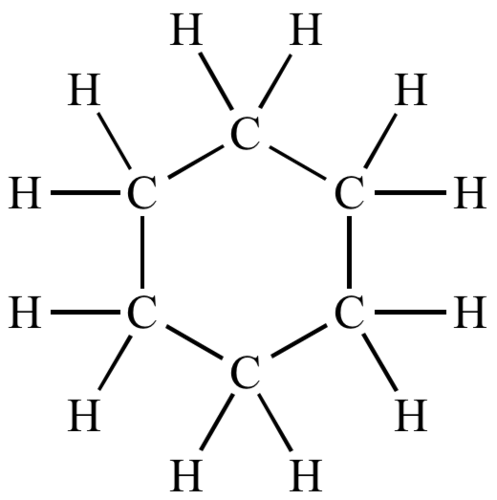
\includegraphics[width=.3\textwidth]{cyclohexane-500x500.png}
    \end{figure}
    \noindent This molecule also has rotational symmetry, but it is a smaller symmetry group than $\mathrm{SO}(2)$. We want to determine this rotational symmetry \emph{subgroup}.
\begin{enumerate}[(a)]
    \item This molecule looks much like a hexagon. Determine the external angles of a hexagon.
    \item Note that if we rotate a hexagon (or cyclohexane) by an external angle, then this leaves the molecule invariant (i.e., it looks no different). Using the internal angle you found, write the rotation matrix for that angle and name this matrix $[g]$.
    \item We can \emph{generate} this group $C_6$ from $[g]$ by repeatedly multiplying $[g]$ with itself.  Show that there are only six elements in this group $C_6$.
    \item These are not all the symmetries of cyclohexane! Explain another symmetry operation that we could use that isn't captured by the rotations above.
\end{enumerate}
If you're interested, look up the group $D_{12}$ which is the \emph{dihedral group of order 12}. Or, taking it further, look at \url{https://en.wikipedia.org/wiki/Cyclohexane_conformation}
\end{problem}
\begin{solution}~
\begin{enumerate}[(a)]
    \item The external angles of a hexagon are $\pi/3$ since the sum of the external angles must be $2\pi$ and there are six angles on a hexagon.
    \item Then we have
    \[
    [g]=\begin{pmatrix} \sqrt{3}/2 & -1/2 \\ 1/2 & \sqrt{3}/2 \end{pmatrix}.
    \]
    \item Now, we can explicitly compute $[g]$, $[g]^2$, $[g]^3$, and so on, but remember that this is a rotation matrix.  Hence, for example, we have
    \[
    \Rot_\theta \Rot_\varphi = \Rot_{\theta+\varphi}.
    \]
    Hence, we have
    \[
    [g]^2 = \Rot_{\pi/3},\quad [g]^3 = \Rot_{\pi/2}, \quad [g]^4 = \Rot_{2\pi/3}, \quad [g]^5 = \Rot_{5\pi/6}, \quad [g]^6 = \Rot_{2\pi}=[I].
    \]
    Indeed, this group does have six elements as there is no way to create any others. This group is known as the \emph{cyclic group of order 6} and we denote it by $C_6$.
    \item The cyclohexane molecule also has reflectional symmetry. That is, we could pick up the molecule, and flip it over (across some axis) and place it back in the same spot. If we include this symmetry as well, we can then generate $D_{12}$. 
\end{enumerate}
\end{solution}

\begin{remark}
The groups $C_n$ and $D_{2n}$ always have this same relationship as the groups $\Orth(n)$ and $\SO(n)$. The idea of rotations and reflections are very related. In fact, reflections are more fundamental in that any rotation is a product of two reflections. This is exactly why we see this relationship.

Also, $\Orth(n)$ and $\SO(n)$ give the reflection/rotation symmetries of $n$-dimensional space. However, we can see that some objects living in those spaces will have smaller symmetry groups. In this case, the group is even finite (order 6) as opposed to infinite!
\end{remark}

\end{document}